% PREAMBLE
\documentclass[a4paper, 12pt, oneside]{article}
\linespread{1.5} %space between lines

\pagestyle{plain}

\usepackage{geometry} %margins
\geometry{a4paper, top=3cm, bottom=3cm, left=3cm, right=3cm, bindingoffset=5mm}


\usepackage{multicol} % multi columns
\usepackage{ragged2e} % text alignment
\usepackage{lmodern} % use modern font style

\usepackage{listings}
\lstset{frame=tb, % listings config, this can be changed in the document body as well
  language=bash,
  aboveskip=3mm,
  belowskip=3mm,
  showstringspaces=false,
  columns=flexible,
  basicstyle={\small\ttfamily},
  numbers=none,
  numberstyle=\tiny\color{SpringGreen},
  keywordstyle=\color{NavyBlue},
  commentstyle=\color{gray},
  stringstyle=\color{Orange},
  breaklines=true,
  breakatwhitespace=true,
  tabsize=3,
  captionpos=b
}

\usepackage{amsmath}
\usepackage[english]{babel} % main language
\usepackage{csquotes}
\usepackage[labelfont=bf]{caption}
\usepackage[backend=biber, style=nature]{biblatex} % bibliography
\addbibresource{biblio.bib}

\usepackage{comment}
\usepackage{xpatch}
\usepackage{blindtext}

\makeatletter

\xpatchcmd{\@makeschapterhead}{%
  \Huge\bfseries  #1\par\nobreak%
}{%
  \Huge \bfseries\centering #1\par\nobreak%
}{\typeout{Patched makeschapterhead}}{\typeout{patching of @makeschapterhead failed}}


\xpatchcmd{\@makechapterhead}{%
  \huge\bfseries \@chapapp\space \thechapter
}{%
  \huge\bfseries\centering \@chapapp\space \thechapter
}{\typeout{Patched @makechapterhead}}{\typeout{Patching of @makechapterhead failed}}

\makeatother

\usepackage{fancyhdr}
\usepackage[export]{adjustbox}

\usepackage{hyperref} % hyperlink
\hypersetup{
    colorlinks=true,
    citecolor=teal,
    linkcolor=black,
    urlcolor=black,
    pdftitle=Master Thesis,
    pdfauthor=Mattia Toninelli,
    }

\usepackage{booktabs}
\usepackage{multirow}
\usepackage[table,xcdraw,dvipsnames]{xcolor}
\usepackage{graphicx}
\graphicspath{ {./figures/} }

\usepackage{lscape}
\usepackage{float}
\usepackage{wrapfig}
% PREAMBLE END

%DOCUMENT START
\begin{document}
\begin{titlepage} % change \vspace{} values for the desired results

  \begin{center}
    
\includegraphics{images/logo.jpg}\par
    \vspace{1cm}
    {\scshape\large GPU Computing Project\par}
    \vspace{4cm}
    {\scshape\large\bfseries Bitonic Sort using Numba on Nvidia GPUs\par}
    \vspace{4cm}
  \end{center}

  \begin{center}
    \scshape\normalsize\textbf{Author:}\\Manuele Lucchi\\08659A \par
  \end{center}

  \vfill

  % Bottom of the page
  {\begin{center}
      \scshape\large Academic Year 2022/2023
    \end{center}}

\end{titlepage}

\section{Abstract}
This documents describe the performances of an existing algorithm, the Bitonic Sort, implemented using Python and Numba, comparing it with a serial approach and CUDA C implementation.

\tableofcontents


\section{Introduction}
The Bitonic Mergesort \cite{bitonic} is an algorithm created in 1968 by Ken Batcher \cite{ken}. The elements to choose for the comparison are indipendent from the value (it's not data-dependant) therefore is well suited for parallel processing.\\
Over the years there are been many implementations using low level languages such as C and even high level such as Java or Python, but regarding the parallel variant, only C/C++ examples can be found on the web (using OpenMP \cite{openmp} and CUDA C \cite{cudac})
The CUDA community developed an abstraction layer over the CUDA runtime to be able to execute CUDA kernels from python with little-to-no overhead using Numba \cite{numba}.\\
Numba is not a CUDA specific framework, it's a generic parallelization abstraction that allows to compile Python functions into machine code, while integrating with numpy \cite{numpy} to have access to a powerful tensor manipulation library;
but of course its primary target is CUDA.\\
The scope of the paper is to implement the algorithm using Numba and compare it with different implementations

\section{Algorithm}

The algorithm is based on the concept of Bitonic Sequence \cite{bitonic}, a sequence with $x_0 \leq ... \leq x_k \geq x ... \geq x_{n-1}$ for some $k$, $0 \leq k \le n$, meaning that there are two subsequences sorted in opposite directions.\\
By using a sorting network, we can create a Bitonic Sequence from any sequence and then merging them to obtain the final sorted sequence, so the algorithm has two phases.\\
This algorithm has an asymptotic complexity of $O(nlog(n)^2)$, the same of the odd-even mergesort \cite{oddeven} and shellsort \cite{shellsort}

\subsection{Step 1: Bitonic Sort}
To create a Bitonic Sequence we need to build a sorting network. This step has $log_2 n$ phases (with the last one being the second step), each one with $i$ stages, where $i$ is the current phase starting from 1.
By sorting each pair of elements in the sequence in different directions pairwise (using the so called "comparers"), we obtain a sequence full of bitonic subsequences. We can then at each phase double the size of these subsequences and half their number.\\
As we can see in picture one, at each stage of a phase the elements in the comparers get closer and in each phase a bitonic subsequence is sorted. This structure is known as butterfly network \cite{butterfly}

\subsection{Step 2: Bitonic Merge}

The last step is a variation of the first one, where we only have a single bitonic sequence and sort the two subsequences with the comparers oriented in the same direction, resulting in the sorted sequence.

\begin{figure}[!h]
  \centering
  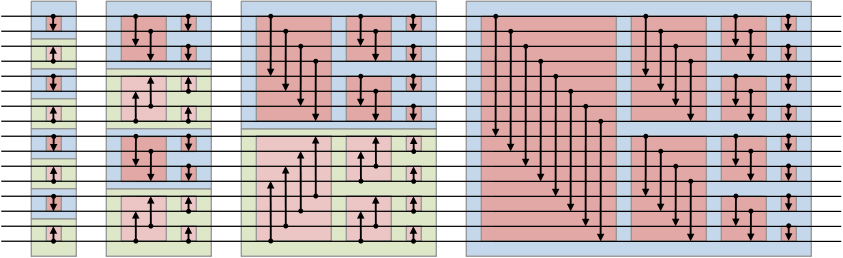
\includegraphics[width= 400pt]{images/bitonic.png}
  \caption{The structure of a bitonic sorting network}
\end{figure}

% versione non potenza di 2 https://hwlang.de/algorithmen/sortieren/bitonic/oddn.htm

\section{Implementation}

The scope of the implementation is to use Numba

% jit tempi compilazione funzione

\subsection{Sequences of length not power of 2}

\section{Benchmark and Profiling}

\begin{center}
  \begin{tabular}{ |c|c|c|c| }
    \hline
    \textbf{Size} & \textbf{CPU Recursive} & \textbf{CPU Iterative} & \textbf{GPU} \\
    \hline
    10            & 10 ms                  & 10 ms                  & 10 ms        \\
    10            & 10 ms                  & 10 ms                  & 10 ms        \\
    \hline
  \end{tabular}
\end{center}

\begin{center}
  \begin{tabular}{ |c|c|c|c| }
    \hline
    \textbf{Size} & \textbf{Cuda C++} & \textbf{Python Numba} \\
    \hline
    10            & 10 ms             & 10 ms                 \\
    10            & 10 ms             & 10 ms                 \\
    \hline
  \end{tabular}
\end{center}

\section{Conclusion}

\printbibliography

\end{document}




